\documentclass{scrartcl}

\usepackage{tabularx} %better tables
\usepackage[table]{xcolor}
\usepackage[utf8]{inputenc}
\usepackage[ngerman]{babel}
\usepackage{hyperref}
\usepackage{tikz}
\usepackage{graphicx}

\begin{document}
	\section*{Realisierungsbericht}
	
	\begin{tabularx}{\textwidth}{| X | X |}
	\hline
	Status & In Arbeit\\
	\hline
	Projektname & DARWIN\\
	\hline
	Projektleiter & Noe Thalheim\\
	\hline
	Auftraggeber & Stefan Schenk\\
	\hline
	Autoren & Yannik Dällenbach, Noe Thalheim\\
	\hline
	\end{tabularx}
	
	\subsection*{Änderungskontrolle}
	\begin{tabularx}{\textwidth}{| X | X | X |}
	\hline
	\rowcolor[gray]{0.9} Version & Datum & Beschreibung\\
	\hline
	1.0 & 12.05.2013 & Init\\
	\hline
	\end{tabularx}
	
	\pagebreak
	%inhaltsverzeichnis
	\tableofcontents
	\pagebreak
	%abschnitt 1
    \section{Zweck des Dokuments}
Zusammenfassung der Ergebnisse der Phase „Realisierung“.
\newpage

	%abschnitt 2
	\section{Technische Detailspezifikation}
\subsection{Innere Struktur}
\subsubsection{Struktur des Systemdesigns}
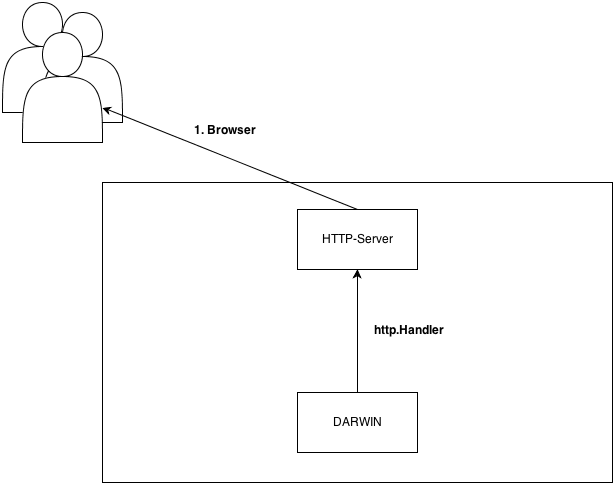
\includegraphics[width=\linewidth]{simplearch.png}
\subsubsection{Beschreibung der Elemente}
Die Architektur von darwin besteht aus 3 Hauptkomponenten.
\subsubsection{Die Spieler}
DARWIN ist ein Multiplayerspiel für bis zu 4 Spieler. Die Spieler können sich via
Netzwerk auf den Server verbinden. Zum Spielen wir ein Browser verwendet.
\subsubsection{Der HTTP-Server}
DARWIN selbst implementiert einen HTTP-Server aus den Standard-Packages von \textbf{go}.
Der HTTP-Server wird für das Hosten der zum Spielen benötigten HTML5-Seiten und
Javascripts verwendet.
\subsubsection{DARWIN (Das Spiel)}
Das Spiel selbst implementiert die allgemeine Spielstruktur welche aus einem Websocket-Server und dem Spiel an sich besteht. Der Websocket-Server implementiert das http.Handler Interface um sich beim HTTP-Server zu registrieren.
\subsection{Schnittstellendefinitionen}
Es werden hauptsächlich zwei Interfaces verwendet.
\subsubsection{1. Browser}
Der Browser stellt die Schnittstelle der Spieler zum Server dar. Diese wurde
mithilfe der Technologien HTML5 und Javascript realisiert.
\subsubsection{http.Handler}
Die http.Handler Schnittstelle wird dazu verwendet eine Methode beim HTTP-Server zu registrieren damit diese per URL-Aufruf ausgeführt wird.
\subsection{Anforderungszuordnung}
%TODO better table an refresh
\begin{tabularx}{\textwidth}{|p{0.7cm}|p{7.0cm}|X|X|}
\hline
Nr. & Anforderung & 1 & 2 \\
\hline
1 & Spielbares Spiel & X & \\
\hline
2 & Lernfähige Gegner & X & X  \\
\hline
3 & Export-Funktion für Gegner & & X  \\
\hline
4 & Bot-Gegen-Bot-Modus & & X    \\
\hline
\end{tabularx}
\newpage

%	\section{Systemanforderungen}

Wir haben uns zuvor bei der Voranalyse mit den Problembereichen unseres Projekts befasst und die Haubtaufgaben bestimmt, diese werden nun detaillierter beschrieben. 


\subsection{Übersicht Anwendungsfälle}

Bei unserem Projekt gibt es grundsätzlich zwei Anwendungsfälle, zum einen die möglichkeit auf dem eigenen System gegen die selbstlernenden Gegener (im folgenden Bots genannt) zu spielen oder einen Bot, der bereits trainiert wurde, zu exportieren und gegen einen Bot eines andern Spieler antretten zu lassen.

\subsection{Spieler gegen Bot}
\begin{tabularx}{\textwidth}{| X | X |}
	\hline
	Kurzbeschreibung & Ein Spieler tritt gegen einen oder mehrere Bots an und versucht gegen diese zu gewinnen. \\
	\hline
	Akteure & Bots und der Spieler. \\
	\hline
	Vorbedingungen & Der Spieler muss über das Proof-Of-Concept verfügen. \\
	\hline
	Ablauf & Der Spieler startet ein neues Spiel.\\
	\hline
	Resultat & Das Spiel wird abgeborchen sobald nur noch der Spieler oder ein Bot am Leben ist. \\
	\hline
	Ausnahmen & In diesem Fall nicht möglich. \\
	\hline	
\end{tabularx}

\subsection{Bot gegen Bot}
\begin{tabularx}{\textwidth}{| X | X |}
	\hline
	Kurzbeschreibung & Zwei Bots tretten gegeneinander an, jeder von ihnen wurde auf einem unabhängigen System trainiert. \\
	\hline
	Akteure & Bot von Spieler eins und Bot von Spieler zwei. \\
	\hline
	Vorbedingungen & Beide Spieler müssen über das Proof-Of-Concept verfügen. \\
	\hline
	Ablauf & Einer der beiden Spieler exportiert sein Bot und übergibt ihm dem anderen Spieler.\\
	\hline
	Resultat & Die beiden Bots spielen in erhöter Geschwindikeit bis einer gewinnt. \\
	\hline
	Ausnahmen & Die Übergabe des Bots fällt nicht in die Verantwortung des Proof-Of-Concept.\\
	\hline
\end{tabularx}

	%abschnitt 3
%	\section{Anforderungszuordnung}

%	\section{Mittelbedarf}
	
\subsection{Sachmittel}
	
Um unser Projekt umzusetzen können wir auf unsere bestehende Hardware zurückgreifen, als Software werden wir Xcode verwenden welches ebenso vorhanden ist. 
Da Xcode über eine native Git-Integration verfügt werden wir als Versionierungssystem Git verwenden und das Repository auf Github
\footnote{Webbasierter Hosting-Dienst für Software-Entwicklungsprojekte, welcher Git als Versionierungssystem verwendet.} hosten. 
\\ \\
Für die Informationsbeschaffung ist es nicht auszuschliessen, dass wir uns im Verlauf des Projekts Bücher kaufen müssen. 
	
\subsection{Personal / Ausbildung}
	
DARWIN befasst sich mit diversen Themen bei denen wir keine oder nur sehr wenig Erfahrung mitbringen. Diese Themen werden wir in Folge des Projekts kennenlernen und uns mit diesen intensiv beschäftigen. 
	
\subsection{Dienstleistung}
Zum jetzigen Zeitpunkt werden wir bei den Dienstleistungen nur auf Git und Github zugreifen.

\subsection{Zeitkontingent}
\begin{tabularx}{\textwidth}{| X | X | X | X |}
\hline
\rowcolor[gray]{0.9} Person & Intern* & Extern** & Total\\
\hline
Thalheim Noe & 60 Stunden & 40 Stunden & 100 Stunden\\
\hline
Dällenbach Yannik & 60 Stunden & 40 Stunden & 100 Stunden\\
\hline
\rowcolor[gray]{0.9} Total & 120 Stunden & 80 Stunden & 200 Stunden\\
\hline
\end{tabularx}
\\
*Intern = Arbeitszeit in der GIBB\\
**Extern = Arbeitszeit ausserhalb der GIBB
\subsection{Finanzielles Budget}
\begin{tabularx}{\textwidth}{| X | X | X | X |}
\hline
\rowcolor[gray]{0.9} Produkt & Preis & Anzahl & Total\\
\hline
Xcode & 0.- & 2 & 0.-\\
\hline
div. Bücher & ca. 100.- & 2 & ca. 200.-\\
\hline
Arbeitszeit* & 0.- & 200 & 0.-\\
\hline
\rowcolor[gray]{0.9} &  & Total & ca. 200.-\\
\hline
\end{tabularx}
\\
*Arbeitszeit wird nicht verrechnet, da sie dem Selbststudium dient.
%	\usetikzlibrary{arrows,positioning}
	
\section{Planung und Organisation}
	
\subsection{Projektorganisation}
An dem Projekt werden folgende Personen mitarbeiten:
\\\\
\begin{tikzpicture}[node distance=1cm, auto]  
\tikzset{
	    mynode/.style={rectangle,align=left,draw=black, top color=white, bottom color=white!50,very thick, inner sep=1em, minimum size=3em, text centered},
	    myarrow/.style={->, >=latex', shorten >=1pt, thick},
	    mylabel/.style={text width=7em, text centered} 
	}  
	\node[mynode] (auftraggeber) {\textbf{Auftraggeber}\\Stefan Schenk};  
	\node[mynode, below=1cm of auftraggeber] (projektleiter) {\textbf{Projektleiter}\\Noe Thalheim};  
	\node[mynode, right=of projektleiter] (projektmitarbeiter1) {\textbf{Projektmitarbeiter}\\Yannik Dällenbach};


	\draw[myarrow] [<->] (auftraggeber.south) -- (projektleiter.north);	
	\draw[myarrow] [-] (projektleiter.east) -- (projektmitarbeiter1.west);

	\end{tikzpicture} 
	\medskip

	Die Aufgabenverteilung wird das ganze Projekt gleich bleiben.
	
	\subsection{Termine}
	
	Für unser Projekt sind folgende Termine von Wichtigkeit:
	\begin{description}
		\item[] Starttermin: 05.02.2013
		\item[] Endtermin: 04.06.2013
	\end{description}
	Daraus ergibt sich für unser Projekt folgender Terminplan:
	\\ \\
	\tiny{
	\begin{tabular}{| p{2cm} | p{1cm} | p{1cm} | p{1cm} | p{1cm} | p{1cm} | p{1cm} |}
	\hline
	\rowcolor[gray]{0.9}  & 12.02.13 - 19.02.13 & 19.02.13 - 05.03.13 & 5.03.13 - 19.03.13 & 19.03.13 - 07.05.13 & 7.05.13 - 21.05.13 & 21.05.13 - 04.06.13 \\
	\hline
	Initialisierung & \cellcolor{yellow} & & & & & \\
	\hline
	Voranalyse & &  \cellcolor{yellow}& & & & \\
	\hline
	Konzept & & &  \cellcolor{yellow}& & & \\
	\hline
	Realisierung & & & &  \cellcolor{yellow}& & \\
	\hline
	Einführung & & & & & \cellcolor{yellow}& \\
	\hline
	Abschluss & & & & &  &\cellcolor{yellow} \\
	\hline
	\end{tabular}	
	}
	\small{
	\\ \\
	Unser Aufgabenplanung werden wir folgendermassen gestalten: 

	\begin{figure}[htb]

	\centering

	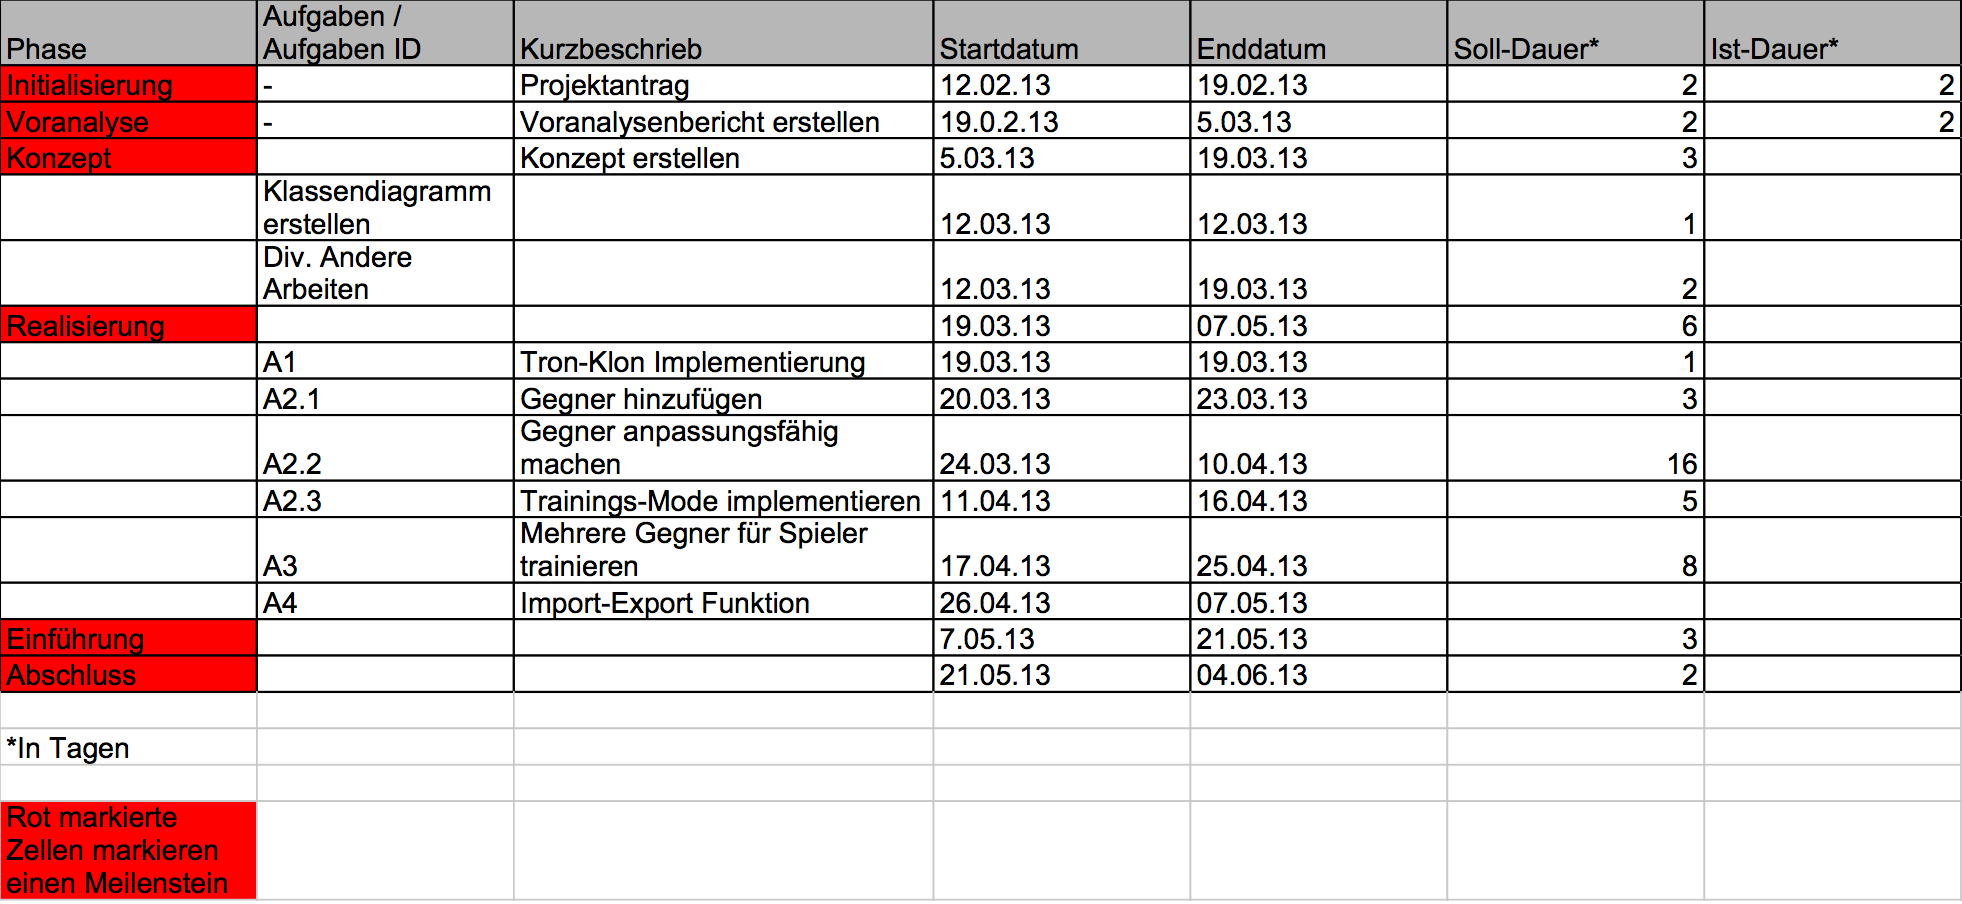
\includegraphics[width=\textwidth]{plan.png}

	\caption{Momentane Aufgabenplanung}

	\end{figure}

	\subsection{Prioritäten}
	Unsere Prioritäten für dieses Projekt sind das Verstehen und Implementieren von Evolutionären Algorithmen und somit das Selbststudium in diesen Gebieten. Zudem ist es uns wichtig durch dieses Projekt Erfahrungen im Zusammenhang mit der Programmierung in Objective-C sammeln zu können. 
}
%	\section{Wirtschaftlichkeit}
	DARWIN soll in einem Proof of Concept aufzeigen wie sich Evolutionäre Algorithmen bewähren, Gegner in einem Spiel dem Spieler anzupassen. Das Projekt hat keinen wirtschaftlichen Aspekt im allgemeinen Sinne, könnte jedoch als Grundlage für ein späteres Projekt dienen.
%	\section{Konsequenzen und Risiken}
\subsection{Risikobeurteilung}
Da es sich bei unserem Projekt um Themen handelt, bei denen keines der Projektmitglieder auf grosse Erfahrung bauen kann ist das grösste Risiko, dass wir Probleme mit der Realisierung der Evolutionären Algorithmen haben werden und somit unser Proof of Concept nicht fertigstellen könnten. Den Tron-Klon auf welchem unser Proof of Concept basiert, können wir hingegen ohne grossen Aufwand realisieren.

\subsection{Ausweichmöglichkeiten}
Falls es tatsächlich soweit kommen sollte, dass es uns nicht möglich ist die von uns erwähnten Evolutionären Algorithmen zu implementieren werden wir uns Hilfe von aussenstehenden organisieren oder die Evolutionären Algorithmen weglassen und uns auf den Tron-Klon konzentrieren. 
%	\pagebreak
\section{Antrag}
	Wir beantragen die Genehmigung des vorliegenden Voranalyseberichts und die Freigabe für die Phase Konzept durch den Auftraggeber.
	\\ \\ \\
	Noe Thaleim:
	\\ \\
	\parbox{4cm}{\hrule
	\strut \centering\footnotesize Ort, Datum} \hfill\parbox{4cm}{\hrule
	\strut \centering\footnotesize Unterschrifft}
	\\ \\ \\
	Yannik Dällenbach:
	\\ \\
	\parbox{4cm}{\hrule
	\strut \centering\footnotesize Ort, Datum} \hfill\parbox{4cm}{\hrule
	\strut \centering\footnotesize Unterschrifft}
	\\ \\ \\
	Für den Auftraggeber:
	\\ \\
	\parbox{4cm}{\hrule
	\strut \centering\footnotesize Ort, Datum} \hfill\parbox{4cm}{\hrule
	\strut \centering\footnotesize Unterschrifft}
\end{document}
